\RequirePackage{lineno}
\RequirePackage{rotating}
\documentclass[12pt]{article}
\usepackage[utf8]{inputenc}
\usepackage{fullpage}
\usepackage[T1]{fontenc}
\usepackage{amsmath, amsthm, amssymb,amsfonts}
\usepackage{mathptmx}
\usepackage{mathtools}
\usepackage{graphicx}
\usepackage{authblk} % To add authors' affiliations
\usepackage[absolute,overlay]{textpos}
\usepackage{braket}  % bra-ket notation
\usepackage{slashed} % Dirac notation
\usepackage{tikz-feynman,contour}
\usepackage{breqn}   % Equation breaking
% Should I use SIUnitX instead?
\usepackage{units}
\usepackage{multirow}
\usepackage{colortbl}
\usepackage{pdflscape} % for sideways figures

\usepackage{hyperref}
\hypersetup{colorlinks,
            citecolor=blue,
            filecolor=black,
            linkcolor=black,
            urlcolor=black
}

\title{Measurement of the neutrino magnetic moment at the NOvA experiment\\ \vspace*{1cm} \texttt{Technical note}}
\author[1]{Robert Kralik}
\affil[1]{University of Sussex, Brighton, UK}
\date{\today}

%\usepackage[printwatermark]{xwatermark}
%\newwatermark[allpages,color=black!20,angle=45,scale=2,xpos=0,ypos=0]{WORK IN PROGRESS}

\usepackage{hyperref}
\hypersetup{
    colorlinks,
    citecolor=blue,
    filecolor=black,
    linkcolor=black,
    urlcolor=black
}

\linenumbers % Include line numbers

\newcommand{\todo }[1]{({\color{red}\sc TO DO: \textit{#1}})}

\begin{document}
\maketitle

\begin{abstract}
    This is the abstract
\end{abstract}
\newpage
\tableofcontents
\newpage

\section{Introduction}

\todo{Describe the main motivations for the analysis. Briefly mention that there was a previous study by Biao, what were the results there and what limitations (or maybe talk about this in the Experimental overview?)}

%The same types of experimental measurements are also sensitive to more exotic neutrino electromagnetic properties: magnetic moments and millicharges, which would be certainly due to new physics beyond the Standard Model. The discovery of millicharges or anomalously large neutrino magnetic moments would have also important implications for astrophysics and cosmology. [NeutrinoPropertiesSnowmass2022.pdf]

%neutrino electromagnetic interactions [...] provide powerful tools to probe the physics beyond the standard model. ... Hence, the theoretical and experimental study of neutrino electromagnetic interactions is a powerful tool in the search for the fundamental theory beyond the standard model. Moreover, the electromagnetic interactions of neutrinos can generate important effects, especially in astrophysical environments, where neutrinos propagate over long distances in magnetic fields in vacuum and in matter. Unfortunately, in spite of many efforts in the search of neutrino electromagnetic interactions, up to now there is no positive experimental indication in favor of their existence. However, it is expected that the standard model neutrino charge radii should be measured in the near future. This will be a test of the standard model and of the physics beyond the standard model which contributes to the neutrino charge radii. Moreover, the existence of neutrino masses and mixing implies that neutrinos have magnetic moments. Since their values depend on the specific theory which extends the standard model in order to accommodate neutrino masses and mixing, experimentalists and theorists are eagerly looking for them. [nuElmagInt2015.pdf]

%The importance of neutrino electromagnetic properties was first mentioned by Pauli in 1930, when he postulated the existence of this particle and discussed the possibility that the neutrino might have a magnetic moment (Pauli, W., 1991, Cambridge Monogr. Part. Phys., Nucl. Phys., Cosmol. 1, 1.). [nuElmagInt2015.pdf]

%Systematic theoretical studies of neutrino electromagnetic properties started after it was shown that in the extended standard model with right-handed neutrinos the magnetic moment of a massive neutrino is, in general, nonvanishing and that its value is determined by the neutrino mass (Lee and Shrock, 1977; Marciano and Sanda, 1977; Petcov, 1977; Fujikawa and Shrock, 1980; Pal and Wolfenstein, 1982; Shrock, 1982; Bilenky and Petcov, 1987). Neutrino electromagnetic properties are important because they are directly connected to fundamentals of particle physics. For example, neutrino electromagnetic properties can be used to distinguish Dirac and Majorana neutrinos, because Dirac neutrinos can have both diagonal and offdiagonal magnetic and electric dipole moments, whereas only the off-diagonal ones are allowed for Majorana neutrinos (Schechter and Valle, 1981; Kayser, 1982, 1984; Nieves, 1982; Pal and Wolfenstein, 1982; Shrock, 1982). Another important case in which Dirac and Majorana neutrinos have quite different observable effects is the spin-flavor precession in an external magnetic field discussed in Sec. VI.B. Neutrino electromagnetic properties are also probes of new physics beyond the standard model, because in the standard model neutrinos can have only a charge radius. The discovery of other neutrino electromagnetic properties would be a signal of new physics beyond the standard model (Bell et al., 2005, 2006; Bell, 2007; Novales-Sanchez et al., 2008). [nuElmagInt2015.pdf]

%Considering an experiment which does not observe any effect of neutrino magnetic moment and obtains a limit on the neutrino mag. moment, it is possible to obtain, following Studenikin (2014), a bound on neutrino millicharge by demanding that the effect of neutrino millicharge is smaller that tha of neutrino magnetic moment. [nuElmagInt2015.pdf - page 580]


%Neutrino electromagnetic properties have been proposed since the very beginning by Pauli to solve the discrepancies in the electron beta emission spectra. This was solved by discovering the neutron. Then again, neutrino magnetic moment was proposed as one of the solution to the solar neutrino problem 

\subsection{Electromagnetic properties of the neutrino}

%In the Standard Model (SM) neutrinos are electrically neutral and do not interact with photons at the tree level. However, radiative corrections generate neutrino interactions with photons through loops involving the charged leptons and the W boson, as shown by the one-loop diagrams in Fig. 9(a). The corresponding neutrino-photon interactions are described by charge radii of the flavor neutrinos . Therefore, even in the SM, where neutrinos are neutral and massless, there are non-zero neutrino electromagnetic properties. [NeutrinoPropertiesSnowmass2022.pdf]

% Although in the standard model neutrinos are electrically neutral and do not possess electric or magnetic dipole moments, they have a charge radius which is generated by radiative corrections. [...] In many extensions of the standard model neutrinos also acquire electromagnetic properties through quantum loop effects which allow direct interactions of neutrinos with electromagnetic fields and electromagnetic interactions of neutrinos with charged particles. Hence, the theoretical and experimental study of neutrino electromagnetic interactions is a powerful tool in the search for the fundamental theory beyond the standard model. Moreover, the electromagnetic interactions of neutrinos can generate important effects, especially in astrophysical environments, where neutrinos propagate over long distances in magnetic fields in vacuum and in matter. [nuElmagInt2015.pdf]

% ...the existence of neutrino masses and mixing implies that neutrinos have magnetic moments. Since their values depend on the specific theory which extends the standard model in order to accommodate neutrino masses and mixing, experimentalists and theorists are eagerly looking for them. [nuElmagInt2015.pdf]

In the standard model, neutrino can have electromagnetic interaction only at a higher order of the perturbative expansion of the interaction - from loop diagrams. 
%But this is only the neutrino charge radius, not the neutrino electric or magnetic moment

%Various theories beyond the Standard Model 
In the one photon approximation, the electromagnetic interactions of a neutrino field $\left(\nu_k\left(x\right), k\in\left\lbrace 1,...,N\right\rbrace\right)$, for $N$ neutrino mass states, can be described by the effective interaction Hamiltonian \cite{nuElmagInt2015.pdf}
\begin{equation}
\mathcal{H}^{\left(\nu\right)}_{em}\left(x\right)=\sum^N_{k,j=1}\overline{\nu}_k\left(x\right)\Lambda^{kj}_{\mu}\nu_j\left(x\right)A^{\mu}\left(x\right)
\end{equation}
and the amplitude of neutrino-to-neutrino interaction for \textbf{Dirac} neutrinos shown on fig.\ref{figFeynman} is
\begin{equation}
\braket{\nu_f\left(p_f\right)|j^{\left(\nu\right)}_{\mu}\left(x\right)|\nu_i\left(p_i\right)}=
e^{i\left(p_f-p_i\right)x}\overline{u}_f\left(p_f\right)\Lambda^{fi}_{\mu}\left(p_f,p_i\right)u_i\left(p_i\right),
\end{equation}
where $p_f$ and $p_i$ are the final and initial four momentums respectively and $u/\overline{u}$ are the solutions to the Dirac equation for a free particle. We take into account possible transitions between different mass states $\nu_i$ and $\nu_f$ \cite{nuElmagInt2015.pdf}.

\begin{figure}
\centering
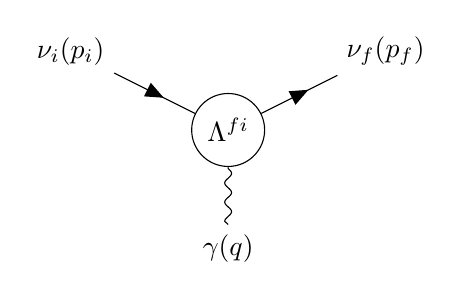
\begin{tikzpicture}
  \begin{feynman}
    \vertex[draw,circle] (m) at ( 0, 0) {$\Lambda^{fi}$};
    \vertex (a) at (-2,1) {\(\nu_i(p_i)\)};
    \vertex (b) at (2,1) {\(\nu_f(p_f)\)};
    \vertex (c) at (0,-1.5) {\(\gamma(q)\)};

    \diagram* {
      (a) -- [fermion] (m) -- [fermion] (b),
      (m) -- [boson] (c)
    };
  \end{feynman}
\end{tikzpicture}
\caption{Effective coupling of neutrinos with one photon electromagnetic field.}
\label{figFeynman}
\end{figure}

The vertex function $\Lambda^{fi}_{\mu}\left(p_f,p_i\right)$ is a matrix and in the most general case it can be written in terms of linearly independent products of Dirac matrices $\left(\gamma\right)$ and four momentum of the photon $\left(q=p_f-p_i\right)$:
\begin{align}
\Lambda^{fi}_{\mu}\left(p_f,p_i\right)=&
\mathbb{F}^{fi}_1\left(q^2\right)q_{\mu}+
\mathbb{F}^{fi}_2\left(q^2\right)q_{\mu}\gamma_5+
\mathbb{F}^{fi}_3\left(q^2\right)\gamma_{\mu}+
\mathbb{F}^{fi}_4\left(q^2\right)\gamma_{\mu}\gamma_5+\notag\\ &
\mathbb{F}^{fi}_5\left(q^2\right)\sigma_{\mu\nu}q^{\nu}+
\mathbb{F}^{fi}_6\left(q^2\right)\epsilon_{\mu\nu\rho\gamma}q^{\nu}\sigma^{\rho\gamma},
\end{align}
where $\mathbb{F}^{fi}_i\left(q^2\right)$ are six Lorentz invariant form factors. For $f=i$ they are called "diagonal" and for $f\neq i$ "transition form factors" \cite{nuElmagInt2015.pdf}.

Applying conditions of hermiticity $\left(\mathcal{H}^{\left(\nu\right)\dagger}_{em}=\mathcal{H}^{\left(\nu\right)}_{em}\right)$ and of conservation of the current (continuity equation: 
$\partial^{\mu}j^{\left(\nu\right)}_{\mu}\left(x\right)=0$), we can rewrite the vertex function as
\begin{equation}
\Lambda^{fi}_{\mu}\left(q\right)=
\left(\gamma_{\mu}-q_{\mu}\slashed{q}/q^2\right)\left[
\mathbb{F}^{fi}_{Q}\left(q^2\right)+\mathbb{F}^{fi}_{A}\left(q^2\right)q^2\gamma_5\right]-
i\sigma_{\mu\nu}q^{\nu}\left[\mathbb{F}^{fi}_{M}\left(q^2\right)+i\mathbb{F}^{fi}_{E}\left(q^2\right)\gamma_5\right],
\end{equation}
where $\mathbb{F}^{fi}_Q,\mathbb{F}^{fi}_M,\mathbb{F}^{fi}_E$ and $\mathbb{F}^{fi}_A$ are hermitian matrices representing the real charge, dipole magnetic, dipole electric and anapole neutrino form factors. In coupling with a real photon $\left(q^2=0\right)$ these become the neutrino charge, magnetic, electric and anapole moment \cite{nuElmagInt2015.pdf}.

For antineutrinos the form factors are transformed as:
\begin{equation}\label{eqAnu1}
\overline{\mathbb{F}}^{fi}_{\Omega}=-\mathbb{F}^{if}_{\Omega}=-\left(\mathbb{F}^{fi}_{\Omega}\right)^{\star} \ \ \ \Omega=Q,M,E,
\end{equation}
\begin{equation}\label{eqAnu2}
\overline{\mathbb{F}}^{fi}_{A}=\mathbb{F}^{if}_{A}=\left(\mathbb{F}^{fi}_{A}\right)^{\star}.
\end{equation}

In case of \textbf{Majorana neutrinos}, the general expression for the vertex function in terms of charge, magnetic, electric and anapole form factors looks the same as for Dirac neutrinos. However, since Majorana antineutrinos are the same particle as Majorana neutrinos, from eq.\ref{eqAnu1},\ref{eqAnu2} we can see that:
\begin{equation}\label{eqAntisymmetryCondition}
\mathbb{F}^M_{\Omega}=-\left(\mathbb{F}^M_{\Omega}\right)^T \ \ \ \Omega=Q,M,E,
\end{equation}
\begin{equation}
\mathbb{F}^M_{A}=\left(\mathbb{F}^M_A\right)^T.
\end{equation}
Therefore the Majorana charge, magnetic and electric form factor matrices are antisymmetric and the anapole form factor matrix is symmetric. This means that Majorana neutrino doesn't have any diagonal charge and dipole magnetic and electric moments, but it can have transition  charge and magnetic and electric moment \cite{nuElmagInt2015.pdf}.

[NuMMBasicsAndAstro\_2022.pdf]
One of the most important for astrophysics consequences of neutrino nonzero effective magnetic moments is the neutrino helicity change $\nu_l\rightarrow\nu_R$ with the appearance of nearly sterile right-handed neutrinos $\nu_R$. In general, this phenomena can proceed in three different mechanisms:
\begin{enumerate}
\item the helicity change in the neutrino magnetic moment scattering on electrons (or protons and neutrons),
\item the neutrino spin and spin-flavour precession in an external magnetic field, and
\item the neutrino spin and spin-flavour precession in the transversally moving matter currents or in the transversally polarized matter at rest
\end{enumerate}
For completeness note that the important astrophysical consequence of nonzero neutrino millicharges is the neutrino deviation from the rectilinear trajectory.

%%%%%%%%%%%%%%%%%%%%%%%%%%%%%%%%%%%%%%%%
\subsubsection{Neutrino electric and magnetic dipole moments}

Evaluating the one loop diagrams in the minimal extension of the standard model with right handed (Dirac) neutrinos gives us the first approximation of the electric and magnetic moments $\left(q^2=0\right)$:
\begin{equation}
\begin{rcases}
\mu^D_{kj}\\
i\epsilon^D_{kj}
\end{rcases}
\simeq\frac{3eG_F}{16\sqrt{2}\pi^2}\left(m_k\pm m_j\right)\left(\delta_{kj}-\frac{1}{2}\sum_{l=e,\mu ,\tau}U^{\star}_{lk}U_{lj}\frac{m_l^2}{m_W^2}\right),
\end{equation}
where $m_k,m_j$ are the neutrino masses, but $m_l$ are the masses of charged leptons which appear in the loop diagrams. Higher order electromagnetic corrections were neglected, but those can also have a significant contribution \cite{nuElmagInt2015.pdf}.

There are no diagonal electric moments $\left(\epsilon_{kk}^D=0\right)$ and the diagonal magnetic moments are approximately
\begin{equation}\label{DiagMagMomVal}
\mu_{kk}^D\simeq\frac{3eG_Fm_k}{8\sqrt{2}\pi^2}\simeq 3.2\times 10^{-19}\left(\frac{m_k}{\textsf{eV}}\right)\mu_B,
\end{equation}
where $\mu_B$ is the Bohr magneton \cite{nuElmagInt2015.pdf}.

The transition magnetic moments are suppressed with respect to the largest of the diagonal magnetic moments by at least a factor of $10^{-4}$ due to the $m_W^2$ in denominator and the transition electric moments are even smaller than that due to the mass difference \cite{nuElmagInt2015.pdf}. Therefore an experimental observation of a magnetic moment larger than in eq.\ref{DiagMagMomVal} would indicate physics beyond the minimally extended standard model \cite{nuMMMajoranaBounds2006.pdf}.

Majorana neutrinos can be obtained by either adding a $\textsf{SU}\left(2\right)_L$ Higgs triplet, or right handed neutrinos together with a $\textsf{SU}\left(2\right)_L$ Higgs singlet. If we neglect the Feynman diagrams which depend on the model of the scalar sector, the magnetic and electric dipole moments are
\begin{equation}
\mu_{kj}^M\simeq -\frac{3ieG_F}{16\sqrt{2}\pi^2}\left(m_k+m_j\right)\sum_{l=e,\mu ,\tau}\operatorname{Im}\left[U^{\star}_{lk}U_{lj}\right]\frac{m_l^2}{m_W^2},
\end{equation}
\begin{equation}
\epsilon_{kj}^M\simeq \frac{3ieG_F}{16\sqrt{2}\pi^2}\left(m_k-m_j\right)\sum_{l=e,\mu ,\tau}\operatorname{Re}\left[U^{\star}_{lk}U_{lj}\right]\frac{m_l^2}{m_W^2}.
\end{equation}
These are difficult to compare to the Dirac case, due to possible presence of Majorana phases in the PMNS matrices, but it is clear that they have the same order of magnitude as Dirac transition dipole moments. However, the neglected model dependent contributions can enhance the transition dipole moments \cite{nuElmagInt2015.pdf}.

It is possible \cite{nuMMMajoranaBounds2006.pdf} to obtain "natural" upper limits on the size of neutrino magnetic moment by calculating its contribution to the neutrino mass by standard model radiative corrections. For Dirac neutrinos the radiative correction induced by neutrino magnetic moment, generated at an energy scale $\Lambda$, to the neutrino mass is generically
\begin{equation}
m_{\nu}^D\sim\frac{\mu_{\nu}^D}{3\times 10^{-15}\mu_B}\left[\Lambda\left(\textsf{TeV}\right)\right]^2\textsf{eV}.
\end{equation}
So for $\Lambda\simeq 1\textsf{TeV}$ and $m_{\nu}\lesssim 0.3\textsf{eV}$ the limit becomes $\mu_{\nu}^D\lesssim 10^{-15}\mu_B$. This applies only if the new physics is well above the electroweak scale ($\Lambda_{EW} \sim 100\textsf{GeV}$). It is possible to get Dirac neutrino magnetic moment higher than this limit, for example in frameworks of minimal super-symmetric standard model, by adding more Higgs doublets, or by considering large extra dimensions \cite{nuElmagInt2015.pdf}.

The limit for Majorana neutrino magnetic moment is less stringent, due to the antisymmetry condition from eq.\ref{eqAntisymmetryCondition} and considering $m_{\nu}\lesssim 0.3\textsf{eV}$ can be expressed as
\begin{align}
\mu_{\tau\mu},\mu_{\tau e} &\lesssim 10^{-9}\left[\Lambda\left(\textsf{TeV}\right)\right]^{-2}\\
\mu_{\mu e} &\lesssim 3\times 10^{-7}\left[\Lambda\left(\textsf{TeV}\right)\right]^{-2}
\end{align}
which is shown in the flavour basis , which relates to the framework used previously as
\begin{equation}
\mu_{ij}=\sum_{\alpha\beta}\mu_{\alpha\beta}U^{\star}_{\alpha i}U_{\beta j},\ \ \ \alpha,\beta\in\left\lbrace e,\mu,\tau\right\rbrace.
\end{equation}
This limits imply, that if a magnetic moment $\mu\gtrsim 10^{-15}\mu_B$ would be measured, it is plausible neutrinos are Majorana fermions and the scale of lepton violation would be well below the conventional see-saw scale \cite{nuMMMajoranaBounds2006.pdf}.

%%%%%%%%%%%%%%%%%%%%%%%%%%%%%%%%%%%%%%%%%%%%%%%%

\subsection{Measuring neutrino magnetic moment}
%Maybe use "Effect of neutrino magnetic moment on measurement" instead
\subsubsection{Effective neutrino magnetic moment}
What we measure in experiments is an effective "flavour" magnetic moment, which is influenced by mixing of "mass" magnetic moments (and electric moments) and oscillations. In the ultrarelativistic limit this is
\begin{equation}
\mu_{\nu_l}^2\left(L,E_{\nu}\right)=\sum_j\left|\sum_k U^{\star}_{lk}e^{-i\Delta m^2_{kj}L/2E_{\nu}}\left(\mu_{jk}-i\epsilon_{jk}\right)\right|^2.
\end{equation}
What is called the effective magnetic moment (often just magnetic moment) therefore contains contributions from both the neutrino magnetic and electric moment \cite{nuElmagInt2015.pdf}.

For antineutrinos, the effective magnetic moment is
\begin{equation}
\mu_{\overline{\nu}_l}^2\left(L,E_{\nu}\right)=\sum_j\left|\sum_k U^{\star}_{lk}e^{+i\Delta m^2_{kj}L/2E_{\nu}}\left(\mu_{jk}-i\epsilon_{jk}\right)\right|^2.
\end{equation}
So the only difference is in the phase induced by neutrino oscillations.

For experiments with baselines short enough for neutrino oscillations to not develop ($\frac{\Delta m^2L}{2E_{\nu}}\ll~1$), such as the NOvA ND, the effective magnetic moment can be expressed as
\begin{equation}
\mu_{\nu_l}^2\simeq\mu_{\overline{\nu}_l}^2\simeq\sum_j\left|\sum_k U_{lk}^{\star}\left(\mu_{jk}-i\epsilon_{jk}\right)\right|^2=\left[U\left(\mu^2+\epsilon^2\right)U^{\dagger}+2\operatorname{Im}\left(U\mu\epsilon U^{\dagger}\right)\right]_{ll^{\prime}},
\end{equation}
which is independent of the neutrino energy and of the source to detector distance.

It is important to mention, that since the effective magnetic moment depends on the flavour of the studied neutrino, it is different for different types of neutrino experiment. Also the solar neutrino experiments need to include the effect of the solar matter on the neutrino oscillations. Therefore the reports on the value (or upper limit) of the effective neutrino magnetic moment are not directly comparable between different types of neutrino experiments.

\subsubsection{Neutrino-on-electron elastic scattering}
The most sensitive method to measure neutrino magnetic moment is the low energy elastic scattering of (anti)neutrinos on electrons \cite{nuElmagInt2015.pdf}. This interaction has two observables, the recoil electron's kinetic energy $\left(T_e\right)$ and the recoil angle with respect to the incoming neutrino beam $\left(\theta\right)$. From simple $2\rightarrow 2$ kinematics we can get
\begin{equation}
\left(P_{\nu}-P_{e^{\prime}}\right)^2=\left(P_{\nu^{\prime}}-P_e\right)^2,
\end{equation}
\begin{equation}
m_{\nu}^2+m_e^2-2E_{\nu}E_{e^{\prime}}+2E_{\nu}p_{e^{\prime}}\cos\theta=m_{\nu}^2+m_e^2-2E_{\nu^{\prime}}m_e.
\end{equation}
Using the energy conservation
\begin{equation}
E_{\nu}+m_e=E_{\nu^{\prime}}+E_{e^{\prime}}=E_{\nu^{\prime}}+T_e+m_e\Rightarrow E_{\nu^{\prime}}=E_{\nu}-T_e
\end{equation}
we get
\begin{equation}
E_{\nu}p_{e^{\prime}}\cos\theta=E_{\nu}E_{e^{\prime}}-E_{\nu^{\prime}}m_e=E_{\nu}\left(T_e+m_e\right)-\left(E_{\nu}-T_e\right)m_e=T_e\left(E_{\nu}+m_e\right),
\end{equation}
\begin{equation}
\cos\theta=\frac{E_{\nu}+m_e}{E_{\nu}}\sqrt{\frac{T_e^2}{E_{e^{\prime}}^2-m_e^2}}=\frac{E_{\nu}+m_e}{E_{\nu}}\sqrt{\frac{T_e^2}{T_e^2+2T_em_e}}.
\end{equation}
And finally we get
\begin{equation}\label{eqThetaTRelation}
\cos\theta=\frac{E_{\nu}+m_e}{E_{\nu}}\sqrt{\frac{T_e}{T_e+2m_e}}.
\end{equation}
Electron's kinetic energy is kinematically constrained by
\begin{equation}
T_e\leq\frac{2E_{\nu}^2}{2E_{\nu}+m_e}.
\end{equation}

Considering $E_{\nu}\sim\textsf{GeV}$, we can approximate $\frac{m_e^2}{E_{\nu}^2}\rightarrow 0$ and in the small angle approximation we get from eq.\ref{eqThetaTRelation} 
\begin{equation}\label{eqTThetaSqExp}
T\theta^2\cong 2m_e\left(1-\frac{T_e}{E_{\nu}}\right)<2m_e.
\end{equation}

In the ultrarelativistic limit, the neutrino magnetic moment changes the neutrino helicity, turning active neutrinos into sterile. Since the SM weak interaction conserves helicity we can add the two contribution to the neutrino on electron cross section incoherently \cite{nuElmagInt2015.pdf}:
\begin{equation}
\frac{d\sigma_{\nu_le^-}}{dT_e}=\left(\frac{d\sigma_{\nu_le^-}}{dT_e}\right)_{\textsf{SM}}+\left(\frac{d\sigma_{\nu_le^-}}{dT_e}\right)_{\textsf{MAG}}.
\end{equation}

The standard model contribution can be expressed as \cite{nuElmagInt2015.pdf}:
\begin{equation}
\left(\frac{d\sigma_{\nu_le^-}}{dT_e}\right)_{\textsf{SM}}=\frac{G_F^2m_e}{2\pi}\left\lbrace\left(g_V^{\nu_l}+g_A^{\nu_l}\right)^2+\left(g_V^{\nu_l}-g_A^{\nu_l}\right)^2\left(1-\frac{T_e}{E_{\nu}}\right)^2+\left(\left(g_A^{\nu_l}\right)^2-\left(g_V^{\nu_l}\right)^2\right)\frac{m_eT_e}{E_{\nu}^2}\right\rbrace,
\end{equation}
where the coupling constants $g_V$ and $g_A$ are different for different neutrino flavours and for antineutrinos. Their values are:
\begin{align}
g_V^{\nu_e}&=2\sin^2\theta_W+1/2,\hspace{2.5cm} g_A^{\nu_e}=1/2,\\
g_V^{\nu_{\mu,\tau}}&=2\sin^2\theta_W-1/2,\hspace{2.25cm} g_A^{\nu_{\mu,\tau}}=-1/2.
\end{align}
For antineutrinos $g_A\rightarrow -g_A$.

Using expressions \ref{eqThetaTRelation} and \ref{eqTThetaSqExp} we can also derive \cite{NuOnECrossSections1989.pdf} cross sections with respect to $\cos\theta$, $\theta^2$ and $T\theta^2$:

\begin{multline}
\left(\frac{d\sigma_{\nu_le^-}}{d\cos\theta}\right)_{\textsf{SM}}=
\frac{2G_F^2E_{\nu}^2m_e^2\cos\theta\left(E_{\nu}+m_e\right)^2}{\pi\left(\left(E_{\nu}+m_e\right)^2-E_{\nu}^2\cos^2\theta\right)^2}\\
\left\lbrace\left(g_V^{\nu_l}+g_A^{\nu_l}\right)^2 +
\left(g_V^{\nu_l}-g_A^{\nu_l}\right)^2\left(1-\frac{2m_eE_{\nu}\cos^2\theta}{\left(E_{\nu}+m_e\right)^2-E_{\nu}^2\cos^2\theta}\right)^2\right. +\\
\left.\left(\left(g_A^{\nu_l}\right)^2-\left(g_V^{\nu_l}\right)^2\right)
\frac{2m_e^2\cos^2\theta}{\left(\left(E_{\nu}+m_e\right)^2-E_{\nu}^2\cos^2\theta\right)}\right\rbrace,
\end{multline}
 
\begin{multline}
\left(\frac{d\sigma_{\nu_le^-}}{d\theta^2}\right)_{\textsf{SM}}=
\frac{G_F^2m_e^2}{\pi\left(\theta^2+\frac{2m_e}{E_{\nu}}\right)^2}
\left\lbrace
\left(g_V^{\nu_l}+g_A^{\nu_l}\right)^2+\left(g_V^{\nu_l}-g_A^{\nu_l}\right)^2
\left(\frac{\theta^2}{\theta^2+\frac{2m_e}{e_{\nu}}}\right)^2\right. +\\
\left.\left(\left(g_A^{\nu_l}\right)^2-\left(g_V^{\nu_l}\right)^2\right)
\frac{2m_e^2}{E_{\nu}^2\left(\theta^2+\frac{2m_e}{E_{\nu}}\right)}\right\rbrace,
\end{multline}

\begin{multline}
\left(\frac{d\sigma_{\nu_le^-}}{dT\theta^2}\right)_{\textsf{SM}}=
\frac{G_F^2E_{\nu}}{4\pi}
\left\lbrace
\left(g_V^{\nu_l}+g_A^{\nu_l}\right)^2+\left(g_V^{\nu_l}-g_A^{\nu_l}\right)^2
\left(\frac{T\theta^2}{2m_e}\right)^2\right. +\\
\left.\left(\left(g_A^{\nu_l}\right)^2-\left(g_V^{\nu_l}\right)^2\right)
\frac{m_e}{E_{\nu}}\left(1-\frac{T\theta^2}{2m_e}\right)\right\rbrace.
\end{multline}

The neutrino magnetic moment contribution is (include derivation from \cite{NeutrinoElmagFormFactors1989.pdf}) \cite{nuElmagInt2015.pdf}:
\begin{equation}
\left(\frac{d\sigma_{\nu_le^-}}{dT_e}\right)_{\textsf{MAG}}=\frac{\pi\alpha^2}{m_e^2}\left(\frac{1}{T_e}-\frac{1}{E_{\nu}}\right)\left(\frac{\mu_{\nu_l}}{\mu_B}\right)^2,
\end{equation}
where $\alpha$ is the fine structure constant.

Analogically to previous, we can also express this cross section in $\cos\theta$, $\theta^2$ and $T\theta^2$:
\begin{equation}
\left(\frac{d\sigma_{\nu_le^-}}{d\cos\theta}\right)_{\textsf{MAG}}=
\frac{2\pi\alpha^2\left(E_{\nu}+m_e\right)^2}{m_e^2\cos\theta}
\frac{\left(E_{\nu}+m_e\right)^2-E_{\nu}^2\cos^2\theta-2m_eE_{\nu}\cos^2\theta}{\left(\left(E_{\nu}+m_e\right)^2-E_{\nu}^2\cos^2\theta\right)^2}
\left(\frac{\mu_{\nu_l}}{\mu_B}\right)^2,
\end{equation}

\begin{equation}
\left(\frac{d\sigma_{\nu_le^-}}{d\theta^2}\right)_{\textsf{MAG}}=\frac{\pi\alpha^2}{m_e^2}\frac{\theta^2}{\left(\theta^2+\frac{2m_e}{E_{\nu}}\right)}\left(\frac{\mu_{\nu_l}}{\mu_B}\right)^2,
\end{equation}

\begin{equation}
\left(\frac{d\sigma_{\nu_le^-}}{dT\theta^2}\right)_{\textsf{MAG}}=\frac{\pi\alpha^2}{4m_e^4}\frac{T\theta^2}{\left(1-\frac{T\theta^2}{2m_e}\right)}\left(\frac{\mu_{\nu_l}}{\mu_B}\right)^2.
\end{equation}

The magnetic moment contribution exceeds the standard model contribution for low enough $T_e$ \cite{nuElmagInt2015.pdf}:
\begin{equation}
T_e\lesssim\frac{\pi^2\alpha^2}{G_F^2m_e^3}\left(\frac{\mu_{\nu}}{\mu_B}\right)^2\simeq 2.9\times 10^{19}\left(\frac{\mu_{\nu}}{\mu_B}\right)^2\left[\textsf{MeV}\right],
\end{equation}
which does not depend on the neutrino energy and makes neutrino experiment sensitive to lower energetic neutrinos more sensitive to the neutrino magnetic moment.
\RequirePackage{lineno}
\documentclass[12pt]{article}
\usepackage[utf8]{inputenc}
\usepackage{fullpage}
\usepackage[T1]{fontenc}
\usepackage{amsmath, amsthm, amssymb,amsfonts}
\usepackage{mathptmx}
\usepackage{graphicx}

\usepackage{hyperref}
\hypersetup{colorlinks,
            citecolor=blue,
            filecolor=black,
            linkcolor=black,
            urlcolor=black
}

\title{Experimental overview of neutrino magnetic moment measurements}
\date{\today}

%\linenumbers % Include line numbers

\begin{document}
\maketitle

\section{Direct muon (anti)neutrino magnetic moment measurements}
\subsection{NOvA (Biao's thesis)}
\begin{itemize}
    \item $\nu_\mu$ only
    \item Only comparing total event counts - 25 events observed and 23.78 expected
    \item Put an upper limit ($90\%$ C.L.) of $\mu_{\nu_\mu}<1.58\times 10^{-9}\mu_B$ with $10.9\%$ systematic uncertainty on the standard model background
    \item Used $3.62\times 10^{20}$ POT of data ($6.74\times 10^{23}$ POT for MC) with $T\theta^2<0.003\textsf{GeV}\times\textsf{Rad}^2$, $0.3<T<0.9\textsf{GeV}$
\end{itemize}

\subsection{MiniBooNE}
\begin{itemize}
    \item $\nu_\mu$ only
    \item Observed excess of events (seems a bit too high)
\end{itemize}

\subsection{E734 at the Alternating Gradient Synchrotron (AGS) of the Brookhaven National Laboratory}
\begin{itemize}
    \item \textbf{Both $\nu_\mu$ and $\overline{\nu}_\mu$}
    \item $\mu_{\nu_\mu}<8.5\times 10^{-10}\mu_B$
%    \item \href{https://journals.aps.org/prd/abstract/10.1103/PhysRevD.41.3297}
\end{itemize}

\subsection{LSND}

\section{Direct electron (anti)neutrino magnetic moment measurements}

\section{Solar neutrino magnetic moment measurements}
\subsection{XENONnT}
First results published in arXiv:2207.11330\cite{XENON:2022mpc} on 22 July 2022.
\begin{itemize}
    \item 5.9 tonne dual-phase liquid xenon TPC dark matter detector
    \item Region Of Interest is (1,140)~keV
    \item Very low background (~5 times lower than XENON1T)
    \item Tritium excluded as the potential background (also in XENON1T)
    \item No excess found - XENON1T excess excluded with ~4$\sigma$
    \item The $90\%$ C.L. upper limit on solar neutrinos with an "enhanced" magnetic moment is \\$\mu_{\nu_{sol}}~<~6.3\times~10^{-12}\mu_B$, the strongest non-astronomical limit so far (see fig.\ref{fig:XENONnTResults})
\end{itemize}

\begin{figure}
    \centering
    \hspace*{1.5cm}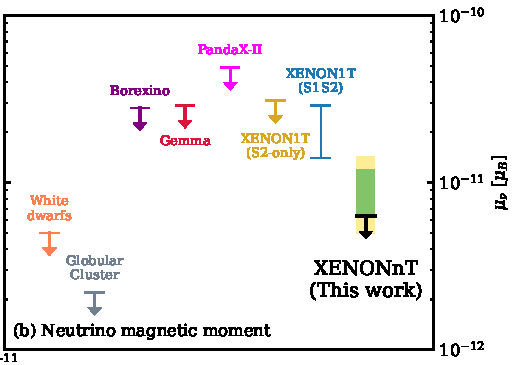
\includegraphics[width=.7\textwidth]{XENONnTExpResultsComparison.pdf}
    \caption{90\% C.L. upper limit on solar neutrinos with an enhanced magnetic moment.}
    \label{fig:XENONnTResults}
\end{figure}
Amir Khan used\cite{Khan:2022bel} XENONnT's results and derived limits on electromagnetic properties for the three SM neutrino flavours (see fig.\ref{fig:XENONnTFit_Khan}).
\begin{figure}
    \centering
    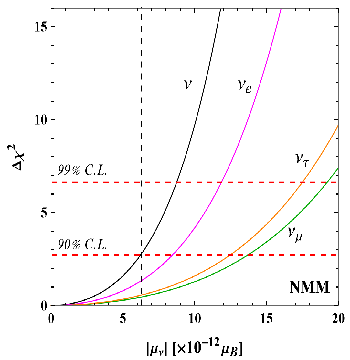
\includegraphics[width=.65\textwidth]{XENONnTFitForNuMM_Khan.pdf}
    \caption{One-dimensional $\Delta\chi^2$ distribution with 90\% and 99\% C.L. boundaries of neutrino magnetic moments. The distribution in black corresponds to the effective flavor independent magnetic moment}
    \label{fig:XENONnTFit_Khan}
\end{figure}
For $\nu_\mu$ they 

\subsection{XENON1T}

\subsection{BOREXINO}

\section{Other}
\subsection{LHC Forward Physics Facilities}
Preliminary sensitivity studies for future experiments (namely for FLArE and FASER$\nu$2)
\begin{itemize}
    \item LHC’s Forward Physics Facilities study high energy (TeV) neutrinos of all flavours from the ATLAS interaction point.
    \item Large opportunity to study tau neutrinos in more detail
\end{itemize}

\bibliographystyle{unsrturl}
\bibliography{ExperimentalOverviewNuMMLiterature}
\end{document}

%%%%%%%%%%%%%%%%%%%%%%%%%%%%%%%%%%%%%%%%%%%%%%%%%%%%%%%%%%%%%%%%%%%%%
%%%                       ANALYSIS OVERVIEW                       %%%
%%%%%%%%%%%%%%%%%%%%%%%%%%%%%%%%%%%%%%%%%%%%%%%%%%%%%%%%%%%%%%%%%%%%%
\section{Analysis overview}
\todo{Describe the motivations for this analysis}
What are we trying to achieve? Are we aiming for purity of the final sample or efficiency of the selection?

We are trying to select nu-on-e events with low electron recoil energies.

\todo{Briefly introduce what are we going to do with these events after the selection (fitting)}
Are we just going to compare the event counts of signal and background (and possibly correct the background based on some other "sideband" selection?), or are we doing a fit to some spectra - either electron energy, angle or ETh2.

\todo{Describe what I'm talking about in this section (datasets, weights, selection, resolution, fitting framework).}

\todo{Describe already here that we're dividing the signal/background into four due to ...}
Here on forward I'm going to describe the differences between these (definitions, weights, signal def, systematics. What is the same: event selection and binning. They're joint together in the fitting framework, where the $\nu_e$CC MEC and the other backgrounds are simply summed together and scaled together. The $\nu$-on-e background (also called the irreducible background by the LDM analysis) is treated/scaled separately.

\textit{Should I describe the NOvA Near Detector here? Specifically its capabilities for detecting electrons?}

\subsection{Datasets and Event Reconstruction details}
For this analysis we are using the near detector samples with a standard Production 5.1 reconstruction. To tackle low number of $\nu$-on-e and $\nu_e$CC MEC events (especially after full selection) in the nominal simulation sample, and to increase speed and lower the computation costs of each study, we are using the following samples for the signal and background components, for the nominal prediction as well as systematically shifted.

\todo{Find out what data sample we're using and write out the data POT}
For data we are only planning to unveil them after fully approved by the collaboration and we will be using the following data sample...

Yiwen has already looked at data for the following samples and the results are here...

Should I mention the POT counting here or somewhere else? - I think I should mention with each separate sample if the POT has to be rescaled or not.

The use of the samples can be briefly summarised as follows:
\begin{table}[!ht]
\centering
\def\arraystretch{1.4}
\begin{tabular}{l@{\hskip 1in}l}
Signal                   & Enhanced $\nu$-on-e sample\\
$\nu$-on-e background    & Enhanced $\nu$-on-e sample\\
$\nu_e$CC MEC background & Enhanced $\nu_e$CC MEC sample\\
Other background         & Nominal ND CAF sample
\end{tabular}
\caption{Overview of simulation samples used.}
\label{tab:DefinitionsOverview}
\end{table}

\subsubsection*{Enhanced $\nu$-on-e sample}
\todo{Describe the nuone sample}
Created by Wenjie Wu (was it just him or also Yiwen?) to do ... and fully described in the technote \cite{NOVA-doc-56383}. Using the overlayed and filematched samples for consistency.

\todo{Find a reference and reasoning for why Wenjie hasn't created the other systematics samples}
We only have the selected few systematics definitions because ... 

\todo{Describe the differences}
\begin{itemize}
\item Missing cross section parameters - unable to use cross section weights or so
\item Special mode for nu-on-e elastic scattering 10005
\end{itemize}

The list of the nu-on-e sample definitions is in table \ref{tab:NuoneDefinitions}.

\begin{table}[!ht]
\centering
\begin{tabular}{p{\textwidth}}
\hline\hline\\
\textbf{Nominal:}\\
\texttt{prod\_caf\_R20-11-25-prod5.1reco.g\_nd\_genie\_N1810j0211a\_nonswap\_fhc\_nova\_v08} \texttt{\_full\_v1\_nuone\_overlay}\\[2mm]
\textbf{Systematically shifted samples:}\\
\texttt{prod\_caf\_R20-11-25-prod5.1reco.g\_nd\_genie\_N1810j0211a\_nonswap\_fhc\_nova\_v08} \texttt{\_full\_calibup\_v1\_nuone\_overlay}\\[2mm]
\texttt{prod\_caf\_R20-11-25-prod5.1reco.g\_nd\_genie\_N1810j0211a\_nonswap\_fhc\_nova\_v08} \texttt{\_full\_calibdown\_v1\_nuone\_overlay}\\[2mm]
\texttt{prod\_caf\_R20-11-25-prod5.1reco.g\_nd\_genie\_N1810j0211a\_nonswap\_fhc\_nova\_v08} \texttt{\_full\_ckvup\_v1\_nuone\_overlay}\\[2mm]
\texttt{prod\_caf\_R20-11-25-prod5.1reco.g\_nd\_genie\_N1810j0211a\_nonswap\_fhc\_nova\_v08} \texttt{\_full\_ckvdown\_v1\_nuone\_overlay}\\[2mm]
\texttt{prod\_caf\_R20-11-25-prod5.1reco.g\_nd\_genie\_N1810j0211a\_nonswap\_fhc\_nova\_v08} \texttt{\_full\_lightlevelup\_v1\_nuone\_overlay}\\[2mm]
\texttt{prod\_caf\_R20-11-25-prod5.1reco.g\_nd\_genie\_N1810j0211a\_nonswap\_fhc\_nova\_v08} \texttt{\_full\_lightleveldown\_v1\_nuone\_overlay}\\[2mm]
\hline\hline
\end{tabular}
\caption{SAMWEB definitions for the $\nu$-on-e samples.}
\label{tab:NuoneDefinitions}
\end{table}

\subsubsection*{Enhance $\nu_e$CC MEC sample}
Created by Yiwen Xiao \cite{NOVA-doc-56383} to tackle the low statistics of the $\nu_e$CC MEC background events and subsequently large and unphysical cross section weights.

\todo{List all the nueCC MEC sample definitions used. Do this after creating the filematched definitions maybe?}

\begin{table}[!ht]
\centering
\begin{tabular}{p{\textwidth}}
\hline\hline\\
\textbf{Nominal:}\\
\texttt{prod\_flatsumdecaf\_R20-11-25-prod5.1reco.g\_nd\_genie\_N1810j0211a\_nonswap\_fhc} \texttt{\_nova\_v08\_full\_v1\_g4rwgt\_respin\_batch2\_filematchedSystematics}\\[2mm]
\textbf{Systematically shifted samples:}\\
\texttt{prod\_flatsumdecaf\_R20-11-25-prod5.1reco.e\_nd\_genie\_N1810j0211a\_nonswap\_fhc} \texttt{\_nova\_v08\_full\_calibdown\_v1\_batch2\_filematchedSystematics\_calibdown\_v1}\\[2mm]
\hline\hline
\end{tabular}
\caption{SAMWEB definitions of the other background samples. THIS IS JUST A PLACEHOLDER!}
\label{tab:NueCCMECDefinitions}
\end{table}

\subsubsection*{Near Detector filematched CAF sample}
\todo{describe and list all the ND nominal CAF samples}

\iffalse
\subsubsection*{Near detector flat summed decaf sample}
What are the cuts used for the DeCAF sample? Why was it created? What is the effect of these cuts?

There's also 3 flavour concats - what are those? there are both numu and nue and they're for the ND... What are the cuts used to create these?

Should I include here also why did I choose to use the decafs instead of cafs? Maybe just point to my talks where I show the plot how much faster it is and that it doesn't matter much for the result. Maybe discuss how different the result would be if I used cafs instead of decafs...

List all the flat sumdecaf definitions used.
\begin{table}[!ht]
\centering
\begin{tabular}{p{\textwidth}}
\hline\hline\\
\textbf{Nominal:}\\
\texttt{prod\_flatsumdecaf\_R20-11-25-prod5.1reco.g\_nd\_genie\_N1810j0211a\_nonswap\_fhc} \texttt{\_nova\_v08\_full\_v1\_g4rwgt\_respin\_batch2\_filematchedSystematics}\\[2mm]
\textbf{Systematically shifted samples:}\\
\texttt{prod\_flatsumdecaf\_R20-11-25-prod5.1reco.e\_nd\_genie\_N1810j0211a\_nonswap\_fhc} \texttt{\_nova\_v08\_full\_calibdown\_v1\_batch2\_filematchedSystematics\_calibdown\_v1}\\[2mm]
\hline\hline
\end{tabular}
\caption{SAMWEB definitions of the other background samples. First figure out what definitions should I use}
\label{tab:SumDeCAFDefinitions}
\end{table}
\fi

\subsection{Analysis weights}
\todo{Describe why do we use weights}
What are the weights we are using and why?

To correct for known deficiencies in simulation of neutrino flux or cross sections we apply weights calculated for each event.

Table \ref{tab:WeightsOverview} shows what CAFAna weights are used to simulate what signal/background sample.

\begin{table}[!ht]
\centering
\def\arraystretch{1.4}
\begin{tabular}{l@{\hskip 1in}l}
Signal                   & Flux and neutrino magnetic moment weights\\
$\nu$-on-e background    & Flux and radiative correction weights\\
$\nu_e$CC MEC background & Flux and cross section weights\\
Other background         & Flux and cross section weights
\end{tabular}
\caption{Overview of CAFAna weights applied to each analysis sample.}
\label{tab:WeightsOverview}
\end{table}

\subsubsection*{PPFX weight}
\texttt{ana::kPPFXFluxCVWgt} \cite{NOVA-doc-23441}
\todo{What does this do (one sentence ish).}

\subsubsection*{Prod5.1 GSF XSec weight}
\texttt{ana::kXSecCVWgt2020GSFProd51}
\todo{Find the reference: possibly Maria's docdb:53336 together with the official 2020 XSec tuning technote docdb:43962.}

\todo{Briefly describe what does this do. Also mention Yiwen's talk/technote about the large XSec weights that made her create an enhanced nueCC MEC sample.}

We are only using the for the background since we assume that the cross section for the signal is perfect. Also there are not weights for this kind of interaction.

\subsubsection*{Radiative correction weight}
\todo{Why are we doing this? (reference Yiwen's talk/technote).}

Mention here where did I get the original GENIE cross section from (reference Yiwen's talk or technote, plus the original paper that was used).

\todo{Write out the actual version of the weight. Including the original and the corrected XSec constants}

Say that we are not using the third part of the correction because it is tiny and it makes no difference. (tried and tested)

\todo{correct the equation}
Calculated as 
\begin{equation}
weight_{\text{Radiative Corr.}} = \left.\frac{d\sigma_{\nu-on-e}}{dy}\right|_{\text{Radiative Corr.}} / \left.\frac{\textsf{d}\sigma_{\nu-on-e}}{\textsf{d}y}\right|_{\text{GENIE 3}};\,y=\frac{E_e-m_e}{E_\nu}
\end{equation}

\subsubsection{Neutrino magnetic moment signal as a weight}
\todo{What does this do and why does it work? Reference the theory part as to why is the magnetic moment signal simply a rescaling of the GENIE cross section.}

Using the same tree-level cross section from GENIE as in the rad. corr. weight.

\todo{Write the name of the weight in CAFAna/nuone namespace and where it is located}

\todo{correct the equation}
Calculated as 
\begin{equation}
weight_{\nu\text{ Mag. Moment}} = \left.\frac{d\sigma_{\nu-on-e}}{dy}\right|_{\nu\text{ Mag. Moment}} / \left.\frac{\textsf{d}\sigma_{\nu-on-e}}{\textsf{d}y}\right|_{\text{GENIE 3}};\,y=\frac{E_e-m_e}{E_\nu}
\end{equation}

\subsection{Event selection}
\textit{Should this be a separate section or is it all right to keep it here? It will have a lot of plots...}

\todo{Add the link to the LDM group's technote and say what's different (or maybe do this after we discuss the cuts?}
Currently we are using the exact same selection as is used by the ND group \cite{NOVA-doc-56383} and very similar to the Light Dark Matter analysis (cite their technote).

\subsubsection*{Signal definition}
\todo{Define the signal of the NuMM. Reference the NuMM weight description above}
The signal of the neutrino magnetic moment analysis is just a reweighted signal of the $\nu$-on-e analysis from the near detector group. We are using the same event selection as the near detector group.

\todo{Decide and explain what signal definitions we're using (kIsVtxContained VS Fiducial volume}
What is the signal and all the background samples definition? Difference between using kIsVtxCont and the fiducial volume. Is there a fundamental difference or preference? Or does it just depend on me? The results/counts are quite different...

\begin{table}[!ht]
\centering
\def\arraystretch{1.4}
\begin{tabular}{p{.25\textwidth}p{.7\textwidth}}
Signal                   & \texttt{kMode}== 10005 \&\& \texttt{NDNuoneFiducial}\\
$\nu$-on-e background    & \texttt{kMode}== 10005 \&\& \texttt{NDNuoneFiducial}\\
$\nu_e$CC MEC background & !(\texttt{kMode}== 5 \&\& \texttt{kElInFinState} \&\& \texttt{NDNuoneFiducial}) \&\& (\texttt{kIsCC} \&\& \texttt{kIsNue} \&\& \texttt{kMode == 10})\\
Other background         & !(\texttt{kMode}== 5 \&\& \texttt{kElInFinState} \&\& \texttt{NDNuoneFiducial}) $||$ !(\texttt{kIsCC} \&\& \texttt{kIsNue} \&\& \texttt{kMode} == 10)
\end{tabular}
\caption{Overview of signal and background definitions. Mode 10005 denotes $\nu$-on-e events, while mode 5 denotes all electron scattering events, including inverse muon decay interactions. That is why we had to add a requirement of an electron in the final state. Mode 10 denotes all MEC events.\todo{Check that the definitions are correct from the code.}}
\label{tab:SignalDefinitions}
\end{table}

\subsubsection*{Pre-selection}

The pre-selection cuts have been kept from the $\nu_e$CC analysis with loosened cut values \todo{find a reference for this analysis}.
Pre-selection cuts include basic quality cuts \todo{describe the basic quality cuts that are implied from the preselection cuts}. They also remove the obvious $\nu$CC interactions by requiring that the length of the longest prong is $<800\ \unit{cm}$, number of planes crossed by the longest prong is $<120$, and the summed number of cells for all prongs in the slice is $<600$. In pre-selection we also include a cut on the time difference between the mean times of the "current" slice and of the slice closest in time, which should be $>25\ \unit{ns}$. This ensures that ... \todo{describe why do we need the closest slice cut with reference to Yiwen's talk and technote}.

%\todo{Add the DeCAF cuts description here - might describe them already when introducing the decaf samples, not sure yet}

\subsubsection*{Fiducial and containment cuts}

\todo{Describe what does the fiducial cut do}
We require that the reconstructed vertex is contained within the following volume: $-185<\textsf{Vtx}_X<175,-175<\textsf{Vtx}_Y<175, 95<\textsf{Vtx}_Z<1095\ \unit{cm}$.

To ensure all the energy is contained within the detector and to remove events originating outside of the detector (rock muons), we require that the extreme positions of hits for all prongs in the slice are within the following volume: $-190<\textsf{min}_X, \textsf{max}_X<180, -180<\textsf{min}_Y, \textsf{max}_Y<190, 105<\textsf{min}_Z, \textsf{max}_Z<1275\ \unit{cm}$

\subsubsection*{Single particle requirement}

To selection events with a single particle we require that the fraction of energy contained in the most energetic shower is $>0.8$, that the summed energy of all cells (above threshold and within $\pm8$ planes from the vertex) outside of the most energetic shower is $<0.02\ \unit{GeV}$, and that the distance between the vertex and the start of the primary shower is $<20\ \unit{cm}$.

\subsubsection*{Shower energy cut}

\todo{discuss the energy cut, should this be removed? What is the effect on the event count? Why was this included in the first place (the identifiers are not as strong for lowere energies - is this true though? - also there are further unexplored backgrounds that would need to be further studied and explore. Maybe depends on where would we move the cut...)}
The calorimetric energy of the primary shower is required to be within $0.5<E_{cal}<5\ \unit{GeV}$.

\subsubsection*{Event classifiers}

We are using two event classifiers based on convolution neural network that were developed specifically to identify $\nu$-on-e interactions. The first one (\texttt{NuoneID}) is trained to select $\nu$-on-e events and the second one (\texttt{Epi0ID}) is trained on the events passing the \texttt{NuoneID} to reject the $\pi^0$ background. Our selection requires that \texttt{NuoneID}$>0.73$ and that \texttt{Epi0ID}$>0.92$.

\todo{reference theory for the kinematics of nuone scattering}
We require that the product of reconstructed energy of the primary shower and the square of its angle from the Z axis is $E_{cal}\theta^2<0.005\ \unit{GeV\times rad^2}$.

\todo{Add plots of distributions of the event selection variables with two columns. LHS shows no cuts applied and RHS shows all previous cuts applied}

Using the many plots below that show the effect of each of the cuts on the signal and all background events. (For signal we are showing NuMM=...)

\todo{Describe the cutflow tables below}
The final event count and efficiency of each of the cuts is shown on the table \ref{tab:CutflowTableSignal}. Table \ref{tab:CutflowTableBackground} shows the dissemination of background into the individual components.

\begin{table}[!hb]
\begin{tabular}{|l|ccc|ccc|ccc|}\hline
\multicolumn{1}{|c|}{}                                     & \multicolumn{3}{c|}{\textbf{$\nu$ Mag. Moment signal}}          & \multicolumn{3}{c|}{\textbf{$\nu$-on-e background}}                      & \multicolumn{3}{c|}{\textbf{Other background}}                           \\
\multicolumn{1}{|c|}{\multirow{-2}{*}{\textbf{Selection}}} & \multicolumn{1}{c}{\textbf{$N_{sig}$}} & \textbf{$\epsilon^{N-1}$} & \textbf{$\epsilon \left(\%\right)$} & \multicolumn{1}{c}{\textbf{$N_{IBkg}$}} & \textbf{$\epsilon^{N-1}$} & \textbf{$\epsilon \left(\%\right)$} & \multicolumn{1}{c}{\textbf{$N_{Bkg}$}} & \textbf{$\epsilon^{N-1}$} & \textbf{$\epsilon \left(\%\right)$} \\\hline
\textbf{No Cut}      & 269.77            & 100 & 100 & 3.43$\times 10^3$           & 100 & 100                                     & 2.96$\times 10^8$          & 100                                                             & 100                                    \\
\textbf{Closest Slc} & 262.20            & 97.19                                                              & 97.19                                     & 3.35$\times 10^3$           & 97.50                                                               & 97.50                                      & 2.74$\times 10^8$          & 92.66                                                              & 92.66                                     \\
\textbf{Png Length} & 169.82            & 64.77                                                              & 62.95                                     & 3.14$\times 10^3$           & 93.72                                                               & 91.38                                      & 7.19$\times 10^7$          & 26.24                                                              & 24.31                                     \\
\textbf{N Planes}       & 169.82            & 100.00                                                             & 62.95                                     & 3.14$\times 10^3$           & 99.98                                                               & 91.37                                      & 7.19$\times 10^7$          & 99.98                                                              & 24.31                                     \\
\textbf{N Cells}        & 169.82            & 100.00                                                             & 62.95                                     & 3.14$\times 10^3$           & 99.98                                                               & 91.35                                      & 6.95$\times 10^7$ & 96.66                                                              & 23.50                                     \\
\textbf{Fiducial}     & 167.72            & 98.76                                                              & 62.17                                     & 3.09$\times 10^3$           & 98.41                                                               & 89.89                                      & 3.59$\times 10^7$          & 51.71                                                              & 12.15                                     \\
\textbf{Cont.}  & 159.37            & 95.02                                                              & 59.08                                     & 2.48$\times 10^3$           & 80.43                                                               & 72.30                                      & 1.38$\times 10^7$          & 38.35                                                              & 4.66                                      \\
\textbf{ShwE Frac.}  & 150.37            & 94.35                                                              & 55.74                                     & 2.42$\times 10^3$           & 97.59                                                               & 70.56                                      & 8.82$\times 10^6$          & 63.97                                                              & 2.98                                      \\
\textbf{Vtx E}         & 142.29            & 94.63                                                              & 52.74                                     & 2.18$\times 10^3$           & 90.16                                                               & 63.62                                      & 4.15$\times 10^6$          & 47.07                                                              & 1.40                                      \\
\textbf{Shw Gap}          & 137.96            & 96.96                                                              & 51.14                                     & 2.09$\times 10^3$           & 95.58                                                               & 60.80                                      & 3.25$\times 10^6$          & 78.34                                                              & 1.10                                      \\
\textbf{Shw E}      & 37.13             & 26.92                                                              & 13.76                                     & 1.36$\times 10^3$           & 65.10                                                               & 39.58                                      & 6.25$\times 10^5$          & 19.21                                                              & 0.21                                      \\
\textbf{Nuoneid}      & 29.48             & 79.39                                                              & 10.93                                     & 940.21             & 69.18                                                               & 27.38                                      & 2.42$\times 10^4$ & 3.88                                                               & 8.19$\times 10^{-3}$                                  \\
\textbf{Epi0id}       & 22.51             & 76.35                                                              & 8.34                                      & 749.93             & 79.76                                                               & 21.84                                      & 1.47$\times 10^4$ & 60.75                                                              & 4.97$\times 10^{-3}$                                  \\
\rowcolor[HTML]{67FD9A}
\textbf{$E\theta^2$}      & 19.74             & 87.73                                                              & 7.32                                      & 675.02             & 90.01                                                               & 19.66                                      & 84.15             & 0.57                                                               & 2.84$\times 10^{-5}$                                 \\\hline\hline
\textbf{$E\theta^2$ (sb)}  & 2.74              & -                                                              & 1.01                                      & 74.30              & -                                                               & 2.16                                       & 1.01$\times 10^3$          & - & 3.43$\times 10^{-4}$                                  \\\hline\hline
\textbf{No ShwE}  & 37.62             & -                                                           & 13.94                                     & 782.67             & -                                                            & 22.79                                      & 238.79            & -                                                              & 8.07E-05   \\\hline
\end{tabular}
\caption{Event selection cutflow table}
\label{tab:CutflowTableSignal}
\end{table}

%\begin{landscape}
\begin{sidewaysfigure}[!hb]
\begin{scriptsize}
%\begin{table}[!hb]
\begin{tabular}{|l|ccc|ccc|ccc|ccc|ccc|}\hline
\multicolumn{1}{|c|}{\multirow{2}{*}{\textbf{Selection}}} & \multicolumn{3}{c|}{\textbf{$\nu_e$CC MEC}} &
\multicolumn{3}{c|}{\textbf{$\nu_e$CC Other}} &
\multicolumn{3}{c|}{\textbf{$\nu_\mu$CC}} &
\multicolumn{3}{c|}{\textbf{NC}} &
\multicolumn{3}{c|}{\textbf{Other}} \\
\multicolumn{1}{|c|}{}                                    & \multicolumn{1}{c}{\textbf{$N$}} & \textbf{$\epsilon^{N-1}$} & \textbf{$\epsilon \left(\%\right)$} & \multicolumn{1}{c}{\textbf{$N$}} & \textbf{$\epsilon^{N-1}$} & \textbf{$\epsilon \left(\%\right)$} & \multicolumn{1}{c}{\textbf{$N$}} & \textbf{$\epsilon^{N-1}$} & \textbf{$\epsilon \left(\%\right)$} & \multicolumn{1}{c}{\textbf{$N$}} & \textbf{$\epsilon^{N-1}$} & \textbf{$\epsilon \left(\%\right)$} & \multicolumn{1}{c}{\textbf{$N$}} & \textbf{$\epsilon^{N-1}$} & \textbf{$\epsilon \left(\%\right)$} \\\hline
\textbf{No Cut}      & 3.50$\times 10^4$           & 100 & 100                                     & 3.23$\times 10^6$             & 100 & 100 & 2.24$\times 10^8$              & 100                                                                 & 100                                        & 3.40$\times 10^7$          & 100.                                                             & 100                                    & 3.49$\times 10^7$                      & 100 & 100                                       \\
\textbf{Closest Slc} & 3.49$\times 10^4$          & 99.78                                                               & 99.78                                      & 2.95$\times 10^6$             & 91.07                                                                 & 91.07                                        & 2.14$\times 10^8$ & 95.45                                                                  & 95.45                                         & 3.16$\times 10^7$                   & 92.81                                                              & 92.81                                     & 2.61$\times 10^7$                      & 74.77                                                                 & 74.77                                        \\
\textbf{Png Length} & 2.73$\times 10^4$           & 78.23                                                               & 78.06                                      & 1.30$\times 10^6$             & 43.99                                                                 & 40.06                                        & 5.51$\times 10^7$          & 25.81                                                                  & 24.64                                         & 1.41$\times 10^7$                   & 44.53                                                              & 41.33                                     & 1.43$\times 10^6$             & 5.49                                                                  & 4.10                                         \\
\textbf{N Planes}       & 2.73$\times 10^4$           & 99.99                                                               & 78.05                                      & 1.30$\times 10^6$             & 99.99                                                                 & 40.06                                        & 5.51$\times 10^7$          & 99.98                                                                  & 24.63                                         & 1.41$\times 10^7$                   & 100.00                                                             & 41.33                                     & 1.43$\times 10^6$             & 100.00                                                                & 4.10                                         \\
\textbf{N Cells}        & 2.73$\times 10^4$           & 99.99                                                               & 78.05                                      & 1.21$\times 10^6$             & 93.29                                                                 & 37.37                                        & 5.33$\times 10^7$          & 96.76                                                                  & 23.84                                         & 1.35$\times 10^7$                   & 96.24                                                              & 39.77                                     & 1.43$\times 10^6$             & 100.00                                                                & 4.10                                         \\
\textbf{Fiducial}     & 1.39$\times 10^4$           & 51.12                                                               & 39.90                                      & 6.30$\times 10^5$ & 52.10                                                                 & 19.47                                        & 2.60$\times 10^7$          & 48.77                                                                  & 11.62                                         & 8.25$\times 10^6$          & 60.99                                                              & 24.26                                     & 1.05$\times 10^6$             & 73.53                                                                 & 3.02                                         \\
\textbf{Cont.}  & 9.32$\times 10^3$           & 66.82                                                               & 26.66                                      & 2.63$\times 10^5$             & 41.72                                                                 & 8.12                                         & 7.64$\times 10^6$              & 29.38                                                                  & 3.42                                          & 4.96$\times 10^6$          & 60.15                                                              & 14.59                                     & 9.12$\times 10^5$             & 86.62                                                                 & 2.61                                         \\
\textbf{ShwE Frac.}  & 9.20$\times 10^3$           & 98.70                                                               & 26.32                                      & 1.95$\times 10^5$             & 74.39                                                                 & 6.04                                         & 4.82$\times 10^6$              & 63.10                                                                  & 2.15                                          & 2.97$\times 10^6$          & 59.78                                                              & 8.72                                      & 8.28$\times 10^5$             & 90.81                                                                 & 2.37                                         \\
\textbf{Vtx E}         & 5.92$\times 10^3$           & 64.33                                                               & 16.93                                      & 6.05$\times 10^4$             & 30.96                                                                 & 1.87                                         & 1.97$\times 10^6$ & 40.79                                                                  & 0.88                                          & 1.36$\times 10^6$          & 45.75                                                              & 3.99                                      & 7.62$\times 10^5$             & 92.03                                                                 & 2.18                                         \\
\textbf{Shw Gap}          & 5.50$\times 10^3$           & 92.91                                                               & 15.73                                      & 4.62$\times 10^4$             & 76.39                                                                 & 1.43                                         & 1.58$\times 10^6$ & 80.18                                                                  & 0.70                                          & 1.06$\times 10^6$          & 77.78                                                              & 3.10                                      & 5.69$\times 10^5$             & 74.61                                                                 & 1.63                                         \\
\textbf{Shw E}      & 3.62$\times 10^3$           & 65.81                                                               & 10.35                                      & 1.12$\times 10^4$             & 24.15                                                                 & 0.35                                         & 4.38$\times 10^5$              & 27.80                                                                  & 0.20                                          & 1.71$\times 10^5$          & 16.15                                                              & 0.50                                      & 1.28$\times 10^3$             & 0.23                                                                  & 3.68$\times 10^{-3}$                                     \\
\textbf{Nuoneid}      & 1.40$\times 10^3$           & 38.63                                                               & 4.00                                       & 2.11$\times 10^3$             & 18.89                                                                 & 0.065                                        & 1.17$\times 10^4$              & 2.66                                                                   & 5.21$\times 10^{-3}$                                      & 8.99$\times 10^3$          & 5.27                                                               & 0.026                                     & 66.43                & 5.17                                                                  & 1.90$\times 10^{-4}$                                     \\
\textbf{Epi0id}       & 1.14$\times 10^3$           & 81.78                                                               & 3.27                                       & 1.61$\times 10^3$             & 76.40                                                                 & 0.050                                        & 7.17$\times 10^3$              & 61.52                                                                  & 3.20$\times 10^{-3}$                                      & 4.76$\times 10^3$          & 52.94                                                              & 0.014                                     & 29.47                & 44.36                                                                 & 8.45$\times 10^{-5}$                                     \\
\rowcolor[HTML]{67FD9A}
\textbf{$E\theta^2$}      & 15.13              & 1.32                                                                & 0.043                                      & 39.00                & 2.42                                                                  & 1.21$\times 10^{-3}$                                     & 8.62                  & 0.12                                                                   & 3.85$\times 10^{-6}$                                      & 20.91             & 0.44                                                               & 6.15$\times 10^{-5}$                                  & 0.50                 & 1.69                                                                  & 1.43$\times 10^{-6}$                                  \\\hline\hline
\textbf{$E\theta^2$ (sb)}  & 386.16             & -                                                            & 1.10                                       & 306.55               & -                                                                & 9.48$\times 10^{-3}$                                     & 165.59                & -                                                               & 7.40$\times 10^{-5}$                                      & 149.93            & -                                                             & 4.41$\times 10^{-4}$                                  & 6.24                 & -                                                              & 1.79$\times 10^{-5}$                                     \\\hline\hline
\textbf{No ShwE}  & 15.54              & -                                                                & 0.044                                      & 69.61                & -                                                                 & 2.15$\times 10^{-3}$                                     & 68.48                 & - & 3.06$\times 10^{-5}$                                      & 75.67             & - & 2.22$\times 10^{-4}$                                  & 9.49                 & -                                                                & 2.72E-05   \\\hline
\end{tabular}
\caption{Event selection cutflow table for background components}
\label{tab:CutflowTableBackground}
%\end{table}
\end{scriptsize}
\end{sidewaysfigure}
%\end{landscape}

\todo{Add a discussion of possible improvements on the event selection on its limitations - mostly for the analysis review committee}
From here we can see that ... Maybe what can be improved is...
This can likely be improved upon by specifically selection low energy events and removing the cut on the reconstructed shower energy. 

\subsection{Resolution and binning}
\todo{Add the energy resolution and binning plots}
The electron energy and angle distributions and resolutions. Are we going to fit in E, Th, or ETh2? Is there something else?

Show plots of Reco V True for both energy and angle. (Should I show it with or without the energy cut?). Also show the resolution plots.

\subsection{Systematic uncertainties}
\todo{Describe the main systematic uncertainties. Add plots showing their effect on the NuMM events. Possibly with different event selection variables as X axes. Also show the final table with the percentages summed}
Plots showing combined uncertainties for signal and backgrounds. Maybe also some interpolations. Table of systematic uncertainties on the event count.

\subsubsection*{Normalization systematics}
\todo{Describe the normalization systematics (or just remove this if not using them in the end}
Should we include normalization systematics? Would that make any difference? There's a POT scaling uncertainty which is very small (find out exactly how small).

In the fitting experiment normalization uncertainties would probably not make any difference whatsoever, but in the counting experiment they might be important?

\subsubsection*{Neutrino flux systematics}
\todo{Describe the flux uncertainties. Describe the PCA. Describe the difference between what the ND group is doing and what we're doing}
Using the PCA vs using the PPFX universes+beam transport separately. Plots of energy showing shifts for signal and backgrounds separately

\todo{understand differences with ND and 3F methods}

This is mainly a normalization. Discuss how to use the fact that $\nu$-on-e events can be used (and are used) to constraint the beam uncertainty. Would the counting experiment still be valid then? Maybe if we made another sideband sample...

\subsubsection*{Detector systematics}
\todo{Make plots of energy showing shifts for signal and backgrounds separately}

\subsubsection*{Cross section systematics}
\todo{Describe the XSec systs}
Only for the non nu-on-e background. Assuming the nu-on-e events (including the signal events) are precisely known.

Plots of energy showing shifts for signal and backgrounds separately

\subsection{Fitting framework}
\todo{Describe the fitting framework, ideally with an example plot, maybe with some arrows}
How does the fitting framework work? It's based on the framework developed by Mu Wei for the Light Dark Matter analysis (ref.) which was developed together (is this fair?). Basic description of the framework.

Also this framework is used for both LDM and NuMM together. It is trivial to simply switch between including the NuMM or LDM in it. This was done to save space in creating predictions since our backgrounds are exactly the same (or at least they should be...). Theoretically this could be separated into two difference frameworks.

\begin{itemize}
\item <NDPredictionSingleElectron> Prediction class which holds the LDM as a special 2-D spectrum (not used for NuMM), and NuMM, $\nu$-on-e background, $\nu_e$CC MEC background and other background as simple 1-D spectra. Also scaling each spectra by...
\item <NDPredictionSystSingleElectron> class derived from PredictionInterp that takes in the NDPredictionSingleElectron and applies systematic shifts to it. Includes the interpolation/extrapolation between the systematic shifts.
\item FitVariables and what do they do
\item Fitter which does exactly what... What are the parameters of the fit? What are the results/outputs?
\end{itemize}
%%%%%%%%%%%%%%%%%%%%%%%%%%%%%%%%%%%%%%%%%%%%%%%%%%%%%%%%%%%%%%%%%%%%%
%%%                           RESULTS                             %%%
%%%%%%%%%%%%%%%%%%%%%%%%%%%%%%%%%%%%%%%%%%%%%%%%%%%%%%%%%%%%%%%%%%%%%
\section{Results / Fake data studies}
[to do]: talk about the shape-only versus normalisation-only strategies for the differential versus single-bin analyses.

I think it might be a good idea to talk about this already in the analysis overview section.

I need to also discuss fake data studies. Should I talk about this now? Probably

\subsection{Counting experiment}
Single bin analysis - total numbers of signal and backgrounds predicted. Possible background corrections and its effect on the background uncertainties. 

\subsection{Binned experiment}
Plots showing delta chi2 for stats and systs separately. Plot showing the chi2 with limits. Maybe talk about using different binning and variables and the effect.

Also need to somehow quantify the various fitter settings, like different seeding values, different range of profiling. Should I talk about Feldman-Cousins? 

\subsubsection{Sensitivities and limits}

\section{Conclusion}
\todo{Report the limit with its uncertainty}

\todo{Very briefly discuss differences with current world limit and how the techniques differ}

\todo{Very briefly summarise expectations for future measurements.}

\bibliographystyle{unsrturl}
\bibliography{NeutrinoMagMomentTechnoteLiterature}
\end{document}
